\documentclass[10pt,letterpaper]{article}
\usepackage[margin=0.66in]{geometry}
\usepackage[T1]{fontenc}
\usepackage{lmodern}
\usepackage{graphicx,booktabs,array}
\usepackage[hidelinks]{hyperref}
\usepackage{fancyhdr}
\pagestyle{fancy}
\fancyhf{}
\fancyhead[L]{\small KUKA PoC figures: verified data and explicit gaps}
\fancyhead[R]{\small 16 October 2026}
\fancyfoot[C]{\thepage}
\setlength{\headheight}{14pt}
\setlength{\parindent}{0pt}
\setlength{\parskip}{5pt}
\setlength{\emergencystretch}{2em}
\renewcommand{\arraystretch}{1.1}
\begin{document}
\section*{KUKA contact-energy guard: what the traces establish}
Results-first adaptation of the original 2-DOF PoC Figures 3--8. The current KUKA reserve/governor policy completes the main blocking fixture and preserves contact, while the frozen endpoint filter exhibits a negative physics energy prefix and substantial contact disturbance. This is a report about the existing implementation; no controller, gains, energy rules or plant parameters were redesigned.


\begingroup
\small
\setlength{\tabcolsep}{4pt}
\renewcommand{\arraystretch}{1.16}
\begin{tabular}{@{}llllll@{}}
\toprule
\textbf{Run} & \textbf{End [s]} & \textbf{Net out [J]} & \textbf{Min raw E [J]} & \textbf{Force peak error [N]} & \textbf{Outcome} \\
\midrule
Main UF & 18 & 0.241623 & -0.1216233 & 0.397 & complete \\
Main A & 18 & 0.119999 & -1.11e-06 & 53.104 & complete \\
Main D & 18 & 0.119591 & 0.0004092 & 1.241 & complete \\
Historical D & 18 & 0.119869 & 8.77e-05 & 1.045 & complete \\
Tiny budget D & 9.533 & 6.86e-05 & 0.0009314 & 0.066 & stopped \\
\bottomrule
\end{tabular}
\endgroup


Energy minima include every executed 0.25 ms physics increment. Force errors use the original 10 N tool/table task target and the declared task window, beginning at 8.71 s. A stopped run contributes only its executed samples; it has no inferred release or recovery.


\begingroup
\small
\setlength{\tabcolsep}{4pt}
\renewcommand{\arraystretch}{1.16}
\begin{tabular}{@{}p{.13\textwidth}p{.80\textwidth}@{}}
\toprule
\textbf{KUKA label} & \textbf{Actual role} \\
\midrule
UF & Matched unfiltered reference; work accounts monitored \\
A & Frozen Stage 1 endpoint joint-torque energy QP \\
B & Physics-prefix energy checks and nonlinear replay \\
C & B plus finite backup reserve, virtual progression and backup selection \\
D & C plus explicit per-stage task acceptance and QP task rows \\
\bottomrule
\end{tabular}
\endgroup


H and R receive the same human work. Archived C and D coincide, and D performs zero recorded QP solves across the 13-case matrix. The supported improvement is therefore evidence for the coupled reserve/governor/backup policy in these fixtures, without establishing active task-QP superiority, independent mismatch accounting or global robot passivity.


\begingroup
\small
\setlength{\tabcolsep}{4pt}
\renewcommand{\arraystretch}{1.16}
\begin{tabular}{@{}lllll@{}}
\toprule
\textbf{13-case matrix} & \textbf{Completed} & \textbf{Stopped} & \textbf{Energy-invalid} & \textbf{Recorded QP calls} \\
\midrule
UF & 13 & 0 & 8 & 0 \\
A & 9 & 4 & 3 & 1354 \\
B & 5 & 8 & 0 & 10 \\
C & 12 & 1 & 0 & 0 \\
D & 12 & 1 & 0 & 0 \\
\bottomrule
\end{tabular}
\endgroup


\clearpage
\section*{Original scientific questions and KUKA coverage}
\begingroup
\small
\setlength{\tabcolsep}{4pt}
\renewcommand{\arraystretch}{1.16}
\begin{tabular}{@{}p{.07\textwidth}p{.14\textwidth}p{.70\textwidth}@{}}
\toprule
\textbf{Family} & \textbf{Status} & \textbf{Supported result and missing comparison} \\
\midrule
F3 & Adapted & No-human task-work exemption/transparency; no closed-loop whole-port baseline \\
F4 & Unsupported & No independently configured mismatch residual; show existing-account identity only \\
F5 & Adapted & Executed blocking power, net/gross work and raw energy for actual KUKA policies \\
F6 & Unsupported & No implemented p\_delta separation; combine the supported identity diagnostic with F4 \\
F7 & Adapted & One continuous help-then-block history; uncapped charging \\
F8 & Adapted & Full coupled-policy interaction/recovery; joint-torque intervention replaces scalar command \\
\bottomrule
\end{tabular}
\endgroup


No family is an exact controller/scenario reproduction. The original 2-DOF plots and raw data establish each question and panel meaning; every result curve here is KUKA data. The complete file/function, signal, units, configuration, adaptation and source-line mapping is recorded in figure\_crosswalk.csv.


\begingroup
\small
\setlength{\tabcolsep}{4pt}
\renewcommand{\arraystretch}{1.16}
\begin{tabular}{@{}p{.23\textwidth}p{.69\textwidth}@{}}
\toprule
\textbf{2-DOF paper label} & \textbf{Actual implementation and relation to KUKA} \\
\midrule
C0 & Nominal; closest experimental role is KUKA UF \\
C1 & Whole-port QP; no KUKA closed-loop equivalent \\
C2 & Residual-only QP; no independent KUKA mismatch/residual equivalent \\
C3 & C3\_dual\_ledger\_qp with governor OFF \\
C4 & The same C3\_dual\_ledger\_qp with governor ON \\
\bottomrule
\end{tabular}
\endgroup


The historical code mode C4\_dual\_ledger\_safe\_scalar is a separate diagnostic and is not paper C4. KUKA C/D labels are unrelated to that naming system. KUKA B versus D changes reserve/governor, backup selection and task protection; it cannot isolate a governor effect.


The main human force acts at a body-fixed link5 point; elbow fixtures use link3. Human power uses velocity at that actual moving point. Tool/table normal contact, its 10 N target and TCP tracking are separate task signals. Positive human power enters the robot; negative power is robot-to-human output. Known force, simulated contact and finite sampled tests remain explicit assumptions.


\clearpage
\section*{F3 --- Task work is exempted, with the causal gap visible}
\begin{center}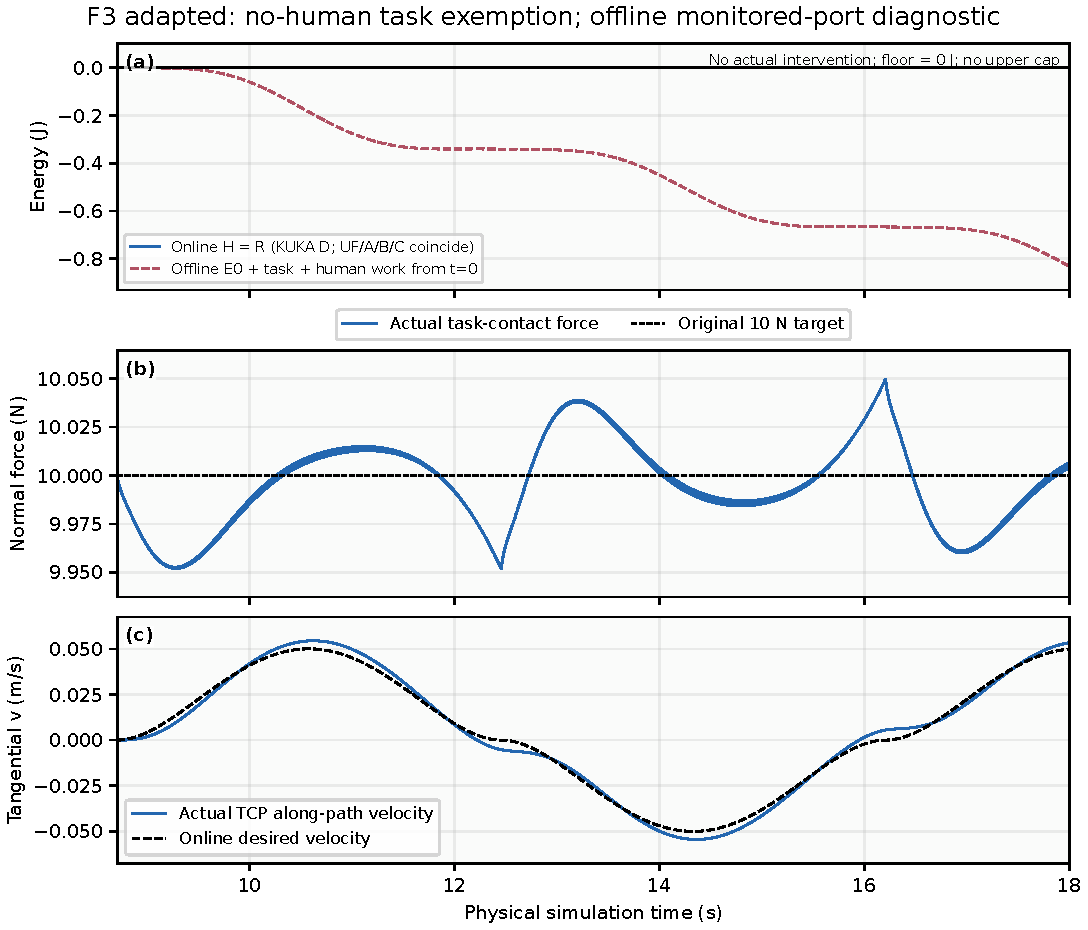
\includegraphics[width=\textwidth,height=6.2in,keepaspectratio]{figures/fig3_task_exemption.pdf}\end{center}
{\small\textbf{F3. No-human task behavior and accounting.} The matched no-human traces show actual ledgers, tool/table normal force and along-path velocity with their implemented floor and references. The offline monitored-port integral starts at t = 0 and includes startup task/contact work before the displayed sliding window, so its initial offset is not attributed solely to useful sliding.}

Zero-initial-energy D preserves the task with E\_H = E\_R = 0 and no actual intervention. The offline diagnostic is not a command-generating whole-port controller, so the original causal claim that useful friction would stop such a controller remains untested for KUKA.


\clearpage
\section*{F4 and F6 --- The current residual account is a copy}
\begin{center}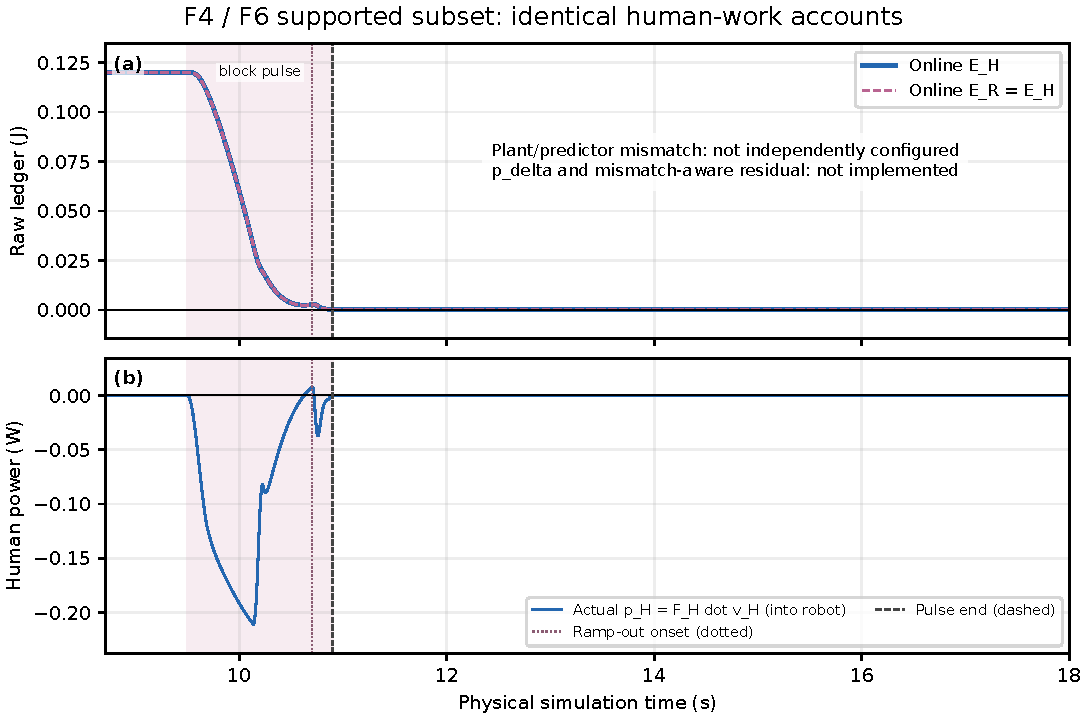
\includegraphics[width=\textwidth,height=5.2in,keepaspectratio]{figures/fig4_fig6_accounting.pdf}\end{center}
{\small\textbf{F4/F6. Supported accounting-identity diagnostic.} Blocking traces, together with no-human F3, expose E\_H = E\_R because both executed accounts receive the same human work. The predictor shares the immutable plant model and holds the currently measured force at its known application point; mismatch power p\_delta is not implemented or replaced with a zero-valued measurement.}

The coincident accounts do not demonstrate mismatch accounting or the original p\_R = p\_H + p\_delta decomposition. Reproducing F4/F6 requires future controller/model work on a physically consistent residual-work meter and independently configured plant/predictor parameters.


\clearpage
\section*{F5 --- Blocking limits signed output, with failures retained}
\begin{center}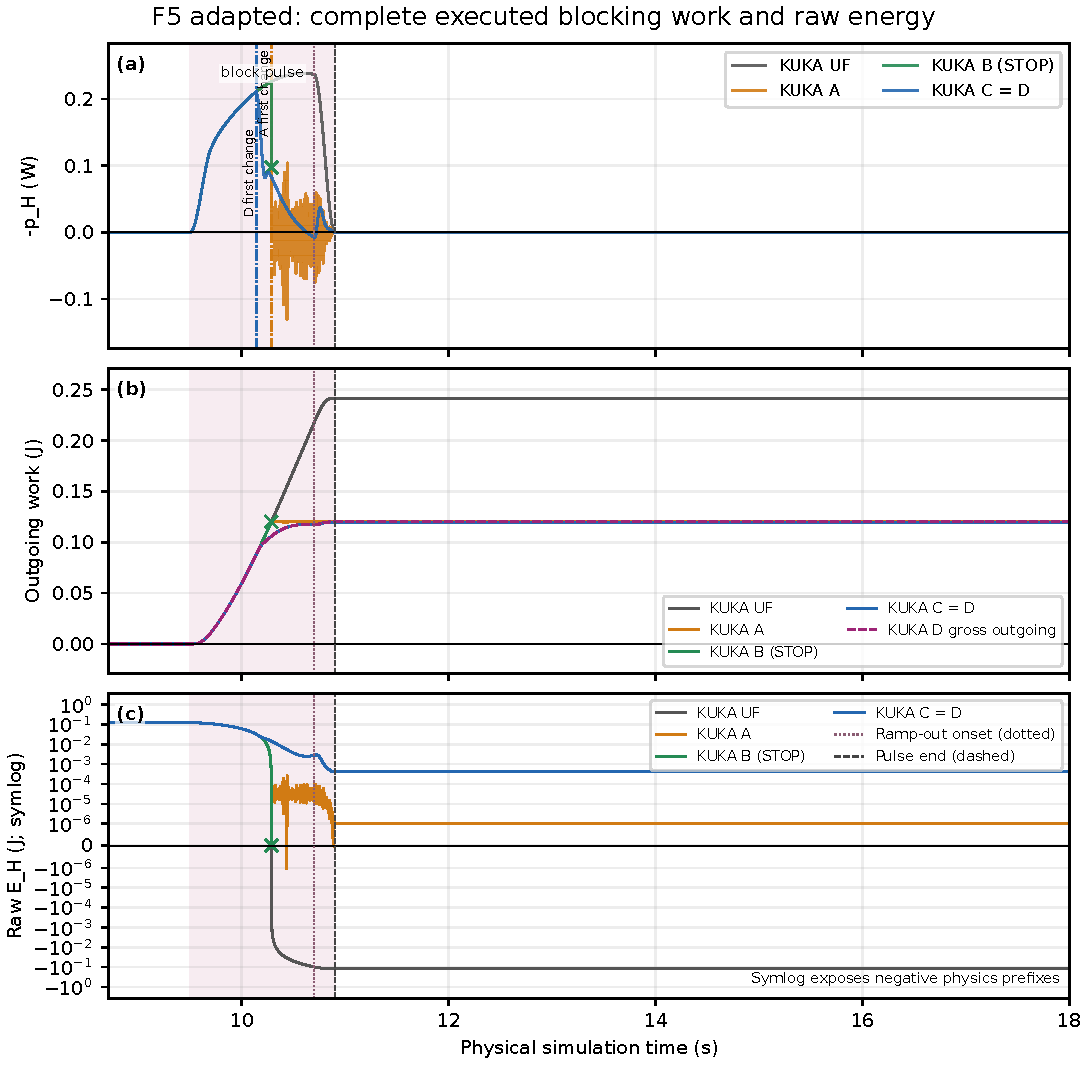
\includegraphics[width=\textwidth,height=6.5in,keepaspectratio]{figures/fig5_blocking.pdf}\end{center}
{\small\textbf{F5. Complete executed blocking power, work and raw energy.} The panels show positive human-directed output -p\_H, signed NET work with gross output identified separately, and raw energy against the implemented zero floor. Ramp-out onset, pulse end, actual intervention and premature termination are distinct events; no unenforced peak-power threshold is drawn.}

Main D finishes with net output 0.119591 J, gross output 0.120004 J and minimum raw energy 0.0004092 J. A reaches a negative physics minimum of -1.11e-06 J despite endpoint checks, while B stops at 10.286 s; these are signed-energy results rather than peak-power, force or gross-work guarantees.


\clearpage
\section*{F7 --- Charging and discharging in one continuous run}
\begin{center}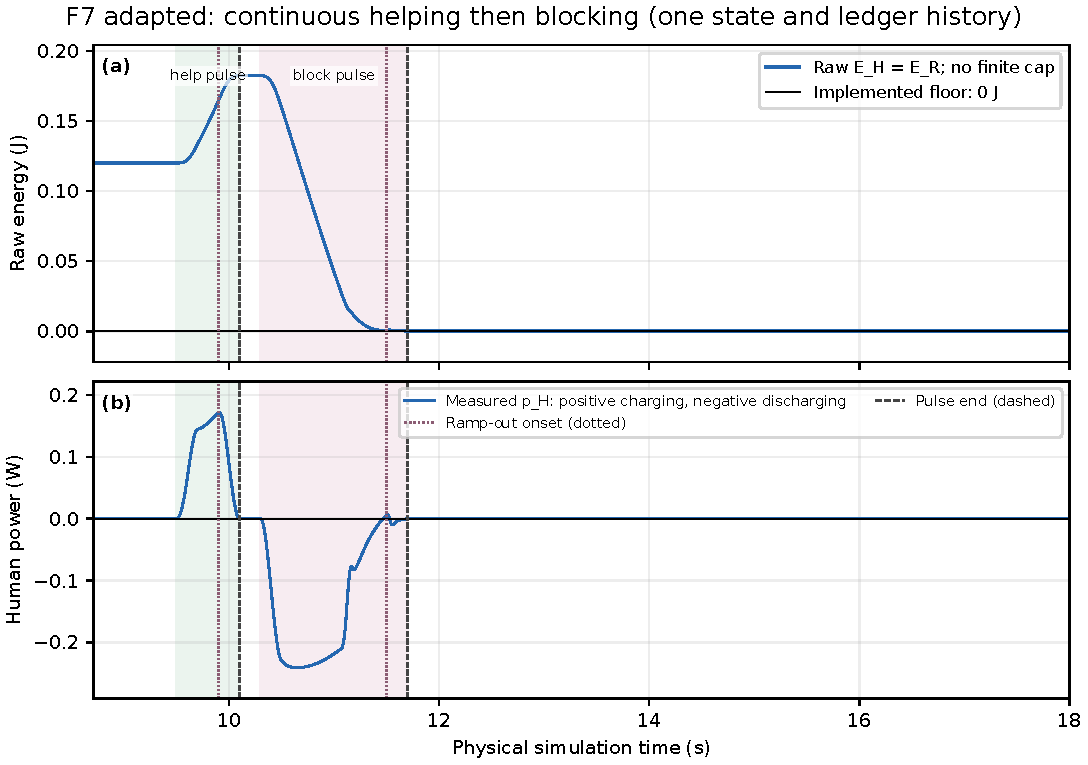
\includegraphics[width=\textwidth,height=5.45in,keepaspectratio]{figures/fig7_charge_discharge.pdf}\end{center}
{\small\textbf{F7. Continuous help-then-block accounting.} The frozen help-then-block profile runs continuously with the same plant, controller, reference history and uncapped ledgers, retaining the implemented zero floor.}

Measured helping work is 0.062228 J, raising energy from 0.12 J to 0.182228 J without clipping; the repeated run matches all executed signals and initial/final states exactly. The run completes at 18 s with net outgoing 0.119849 J, gross outgoing 0.182297 J and minimum raw energy 0.000150544 J. Gross output can exceed the initial budget because measured positive human-point work recharges it, while the implemented constraint concerns signed net work; phase interpretation uses measured power rather than force direction alone.


\clearpage
\section*{F8 --- Complete interaction and recovery of the current policy}
\begin{center}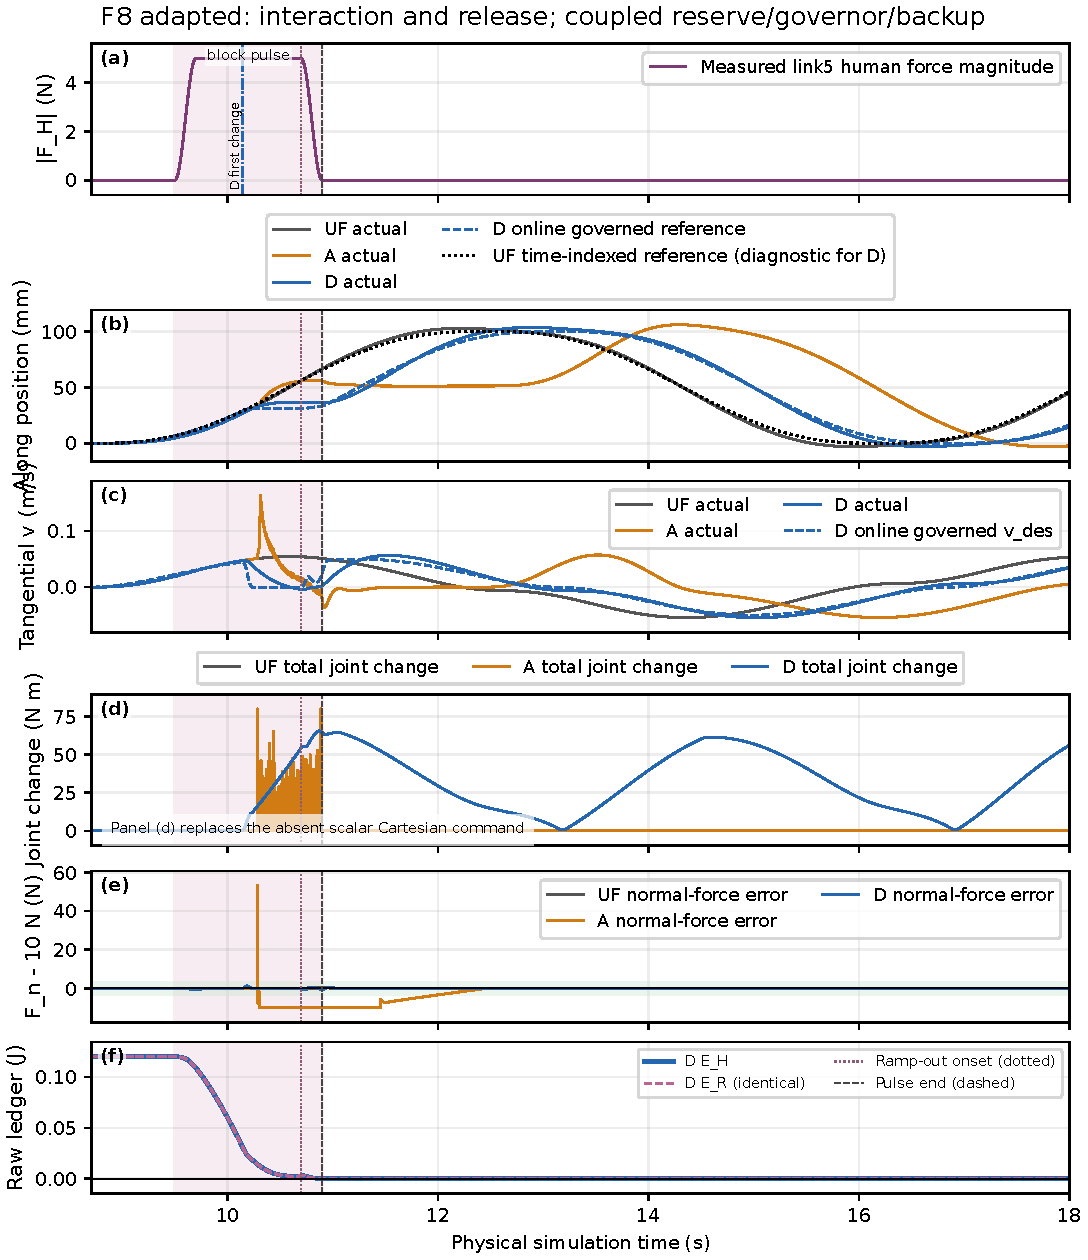
\includegraphics[width=\textwidth,height=6.85in,keepaspectratio]{figures/fig8_recovery.pdf}\end{center}
{\small\textbf{F8. Adapted interaction/recovery comparison.} Six panels retain force/events, actual and online governed position/velocity, original-target force error and raw H/R accounts, with any original-time reference marked diagnostic; panel (d) replaces the absent scalar Cartesian command with joint-torque intervention in N m.}

D starts intervening at 10.14 s; A first intervenes at 10.285 s. Main D sustained force recovery takes 0.262 s from ramp-out onset, or 0.062 s from full force removal, using a full 0.5 s all-good window and explicitly distinguishing the old paper's ramp-out release anchor.


KUKA's virtual clock preserves stroke endpoints rather than capturing the old spatial anchor, and this coupled reserve/governor/backup comparison does not isolate a governor effect.


\clearpage
\section*{Quantitative task, interaction and recovery outcomes}
\begingroup
\small
\setlength{\tabcolsep}{4pt}
\renewcommand{\arraystretch}{1.16}
\begin{tabular}{@{}llllll@{}}
\toprule
\textbf{Main policy} & \textbf{Force RMSE [N]} & \textbf{MAE [N]} & \textbf{Max error [N]} & \textbf{Absent [s]} & \textbf{End [s]} \\
\midrule
UF & 0.074 & 0.04 & 0.397 & 0 & 18 \\
A & 3.838 & 1.691 & 53.104 & 1.14975 & 18 \\
B & 0.482 & 0.103 & 18.439 & 0 & 10.286 \\
C & 0.129 & 0.063 & 1.241 & 0 & 18 \\
D & 0.129 & 0.063 & 1.241 & 0 & 18 \\
\bottomrule
\end{tabular}
\endgroup


These force statistics use each run's executed task interval [8.71 s, actual end). Equal-duration main UF/A/D rows support full-task comparisons; B ends early and its full-run aggregate has a shorter window. No samples are repeated after termination. Maximum errors and contact absence retain the original 10 N target during controller recovery.


\begingroup
\small
\setlength{\tabcolsep}{4pt}
\renewcommand{\arraystretch}{1.16}
\begin{tabular}{@{}llll@{}}
\toprule
\textbf{Common window} & \textbf{Force RMSE [N]} & \textbf{Force MAE [N]} & \textbf{Tangent RMSE [m/s]} \\
\midrule
UF & 0.133 & 0.091 & 0.00257 \\
A & 1.341 & 0.125 & 0.00257 \\
B & 0.482 & 0.103 & 0.00257 \\
C & 0.231 & 0.129 & 0.00918 \\
D & 0.231 & 0.129 & 0.00918 \\
\bottomrule
\end{tabular}
\endgroup


The equal-support table ends at 10.286 s for every main policy. It does not replace the full-run completion and violation outcomes.


\begingroup
\small
\setlength{\tabcolsep}{4pt}
\renewcommand{\arraystretch}{1.16}
\begin{tabular}{@{}lllll@{}}
\toprule
\textbf{Run} & \textbf{Tangent RMSE [m/s]} & \textbf{Peak speed [m/s]} & \textbf{Online debt [mm]} & \textbf{Force recovery [s]} \\
\midrule
Main A & 0.00893 & 0.163 & 5.976 & 1.49 \\
Main D & 0.00756 & 0.0567 & 5.62 & 0.062 \\
Historical D & 0.00826 & 0.0552 & 7.45 & 0.078 \\
\bottomrule
\end{tabular}
\endgroup


\begingroup
\small
\setlength{\tabcolsep}{4pt}
\renewcommand{\arraystretch}{1.16}
\begin{tabular}{@{}lll@{}}
\toprule
\textbf{Run} & \textbf{Peak original-reference debt [mm]} & \textbf{Progress / matched UF [\%]} \\
\midrule
Main A & 77.982 & 81.73 \\
Main D & 32.756 & 87.526 \\
Historical D & 26.974 & 89.363 \\
\bottomrule
\end{tabular}
\endgroup


\begingroup
\small
\setlength{\tabcolsep}{4pt}
\renewcommand{\arraystretch}{1.16}
\begin{tabular}{@{}lllll@{}}
\toprule
\textbf{Run} & \textbf{Net / gross [J]} & \textbf{Peak output [W]} & \textbf{Progress [m]} & \textbf{Outcome} \\
\midrule
Main A & 0.119999 / 0.124648 & 0.226 & 0.2005 & complete \\
Main D & 0.119591 / 0.120004 & 0.211 & 0.2147 & complete \\
Historical A & 0.119977 / 0.119977 & 0.217 & 0.0588 & stopped \\
Historical D & 0.119869 / 0.119927 & 0.217 & 0.2192 & complete \\
Tiny budget D & 6.86e-05 / 6.86e-05 & 0.006 & 0.0054 & stopped \\
\bottomrule
\end{tabular}
\endgroup


Tangential tracking compares actual TCP velocity with the online governed reference at control samples; the peak-speed metric uses physics samples. Online tracking debt, original-reference debt and ordered task-progress loss are distinct declared metrics. Force recovery is measured from pulse end and requires 0.5 s of sustained recovery. The historical A stop and tiny-budget D stop remain failures to complete, even when their executed prefixes satisfy a subset of constraints.


\clearpage
\section*{KUKA supplement --- Reserve, progression, completion and runtime}
\begin{center}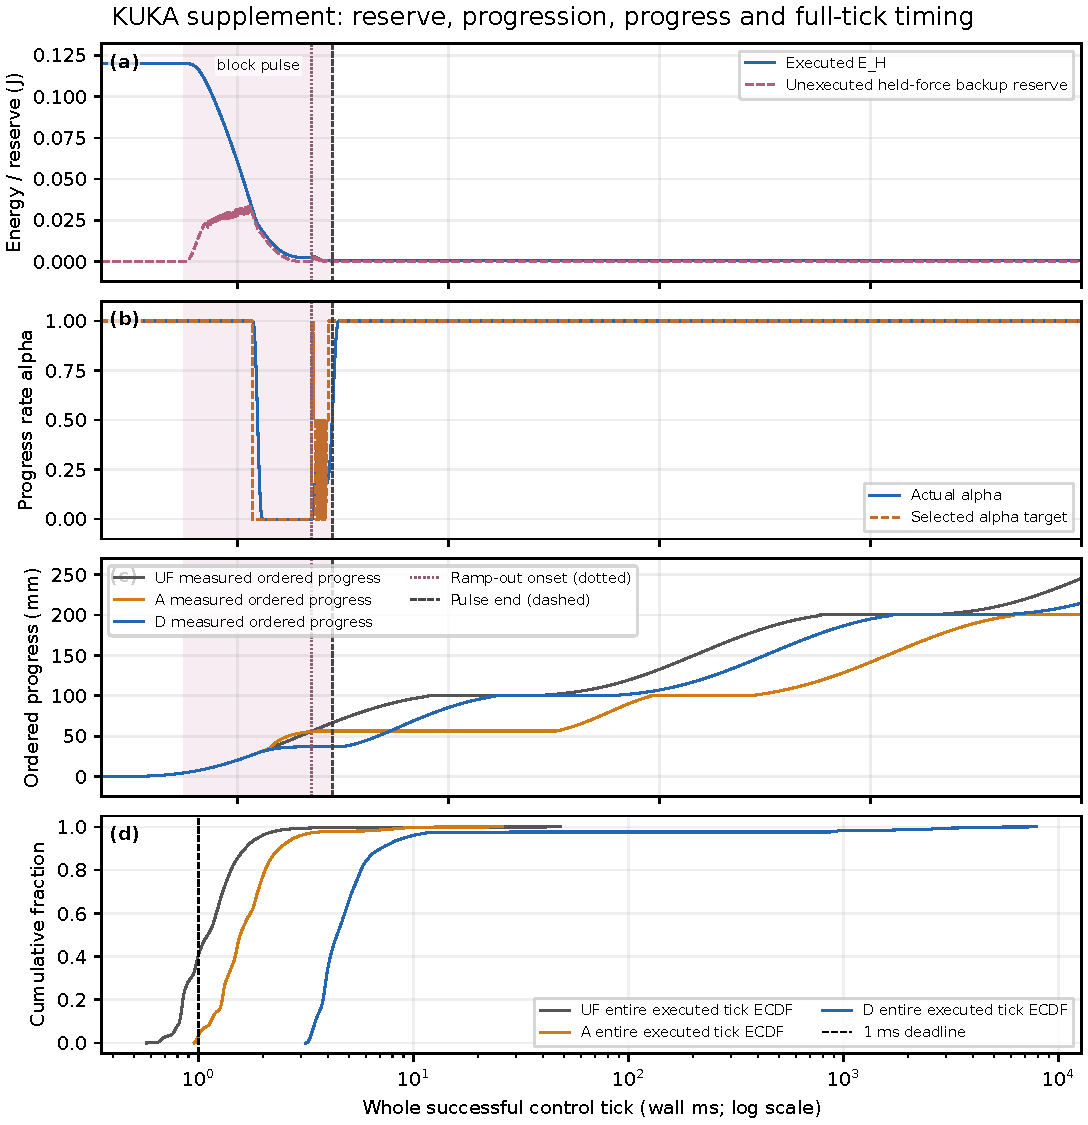
\includegraphics[width=\textwidth,height=4.7in,keepaspectratio]{figures/figS_reserve_progress_timing.pdf}\end{center}
{\small\textbf{KUKA-specific supplement.} Available actual energy and the unexecuted current-held-force backup reserve have different provenance. Alpha target and actual alpha expose transition dynamics. Ordered progress avoids treating back-and-forth displacement as completed work. Whole successful control-tick timing is compared with the 1 ms simulated deadline; timing distributions are not a real-time certificate.}

\begingroup
\small
\setlength{\tabcolsep}{4pt}
\renewcommand{\arraystretch}{1.16}
\begin{tabular}{@{}llll@{}}
\toprule
\textbf{Main policy} & \textbf{Recorded QP calls} & \textbf{Torque correction ticks} & \textbf{Intervention ticks} \\
\midrule
UF & 0 & 0 & 0 \\
A & 334 & 334 & 334 \\
B & 2 & 1 & 1 \\
C & 0 & 626 & 705 \\
D & 0 & 626 & 705 \\
\bottomrule
\end{tabular}
\endgroup


Zero recorded C/D solves or active rows on selected executed paths does not prove that no solver work occurred inside rejected plans: the existing guard discards some attempted-plan timing/diagnostics after a reserve or reaction-path rejection. No active task-QP advantage is inferred from this record.


Main D pauses for 0.482 s and accumulates maximum virtual-time delay 0.669 s. Its ordered measured progress at 18 s is 0.2147 m versus matched UF 0.2453 m. Preserved continuous extensions measure equal-progress completion without resetting the clock, ledgers or controller history.


Additional physical time to reach the matched UF 18 s task amount is main 0.668 s and historical 0.546 s; the reference amount and crossing rule are recorded in the manifest.


Main D successful whole-tick wall time: median 0.004415 s, p99 2.544035 s, maximum 7.916327 s; 18000 measured successful ticks exceed 1 ms. Full forecasts are offline computations, and failures are reported separately. Current measured force is held throughout each prediction; future scripted pulse values are not supplied to the guard.


\clearpage
\section*{Four-round verification, provenance and remaining limits}
\begingroup
\small
\setlength{\tabcolsep}{4pt}
\renewcommand{\arraystretch}{1.16}
\begin{tabular}{@{}p{.06\textwidth}p{.12\textwidth}p{.73\textwidth}@{}}
\toprule
\textbf{Round} & \textbf{Verdict} & \textbf{Recorded evidence} \\
\midrule
1 & PASS & Canonical mapping and independent raw metrics passed; elapsed-zero timestamps, curve provenance and PDF legibility corrected. F7 was pending at this round and completed in Round 3. \\
2 & PASS & All 13 matched fixtures and five transparent fixture families verified; 26 focused tests passed. F3 startup accounting and release-anchor labels corrected. \\
3 & PASS & Reused exact-source main repeat and fresh no-human, stop and repeated continuous runs verified; 597 headline and 30 common-window checks passed. Charging coverage and torque mapping corrected. \\
4 & PASS & Clean build and all 10 PDF pages inspected; four legend/annotation occlusions corrected. Metrics and curve contracts unchanged; scientific claims and preservation verified. \\
\bottomrule
\end{tabular}
\endgroup


Detailed findings, justified corrections, commands, true subprocess exit status and structured test counts are in reviews/round\_01.md through round\_04.md and review\_summary.json. Report correctness is assessed separately from scientific success: an unsupported mismatch mechanism, an inactive task-QP comparison and an explicit stop can be reported correctly.


\begingroup
\small
\setlength{\tabcolsep}{4pt}
\renewcommand{\arraystretch}{1.16}
\begin{tabular}{@{}p{.60\textwidth}p{.31\textwidth}@{}}
\toprule
\textbf{Proposal component} & \textbf{Coverage} \\
\midrule
Known-point signed work; task exemption; finite fixture reserve/recovery & Demonstrated on reported fixtures \\
Continuous bidirectional charging without an upper cap & Demonstrated on the frozen continuous fixture and exact repeat \\
Per-stage task QP & Partially tested; no selected accepted task-QP rows in archived D matrix \\
Whole-port causal baseline; independent mismatch/residual account & Missing \\
Isolated governor ablation; finite ledger cap; peak-power/force protection & Missing \\
Global passivity; arbitrary-force robustness; recursive feasibility; 1 kHz hardware & Not established \\
\bottomrule
\end{tabular}
\endgroup


All plotted physics powers and work increments remain unsmoothed. Actual raw ledgers are never lower-clamped; rejected candidates and unexecuted backup predictions are separated from executed trajectories. The complete manifest maps every curve to its preserved raw file/hash, source/configuration, units, sampling stage, transform and window. Original source, results and reports remain preserved in their prior worktrees.


Starting synchronized Stage 2 source: 41359f20430c930eec5afaebffa2cfbc482f07da. Numerical-source archive: 81dffa64109752a9a027975e7b831daa4ff91e86. New plotting branch: feature/kuka-poc-figures-20261016-41359f2. Final artifact/source hashes and the final Git revision are recorded in the reproducibility and preservation records, avoiding a self-referential commit hash in the PDF.


Reproduction: use the exact single-entry build command in reproduction.md with preserved inputs, a clean new output directory and the four review records. Simulation generation is separate and uses the frozen run configuration. The editable Markdown also preserves the complete command.


\end{document}
